%%%%%%%%%%%%%%%%%%%%%%%%%%%%%%%%%%%%%%%
% Deedy CV/Resume
% XeLaTeX Template
% Version 1.0 (5/5/2014)
%
% This template has been downloaded from:
% http://www.LaTeXTemplates.com
%
% Original author:
% Debarghya Das (http://www.debarghyadas.com)
% With extensive modifications by:
% Vel (vel@latextemplates.com)
%
% License:
% CC BY-NC-SA 3.0 (http://creativecommons.org/licenses/by-nc-sa/3.0/)
%
% Important notes:
% This template needs to be compiled with XeLaTeX.
%
%%%%%%%%%%%%%%%%%%%%%%%%%%%%%%%%%%%%%%

\documentclass[letterpaper]{deedy-resume} % Use US Letter paper, change to a4paper for A4 
\usepackage{hyperref}
\usepackage{calc}
\usepackage{graphicx}
\usepackage{wrapfig}                      %To wrap the text around the image
\definecolor{linkcolour}{rgb}{0.25,0.25,0.6}
\hypersetup{colorlinks,
            linkcolor = linkcolour,
            urlcolor  = linkcolour}
\graphicspath{ {.} }
\begin{document}

%----------------------------------------------------------------------------------------
%	TITLE SECTION
%----------------------------------------------------------------------------------------

%\namesection{R}{Sundararajan}{ % Your name
%\small Third Year Undergraduate, Computer Science and Engineering | \href{mailto:rsundar@cse.iitk.ac.in}{rsundar@iitk.ac.in} | +91-8765674508\\
%}
% \begin{wrapfigure}{r}{1.78in}
% \vspace{-0.36cm}
% \centering
% 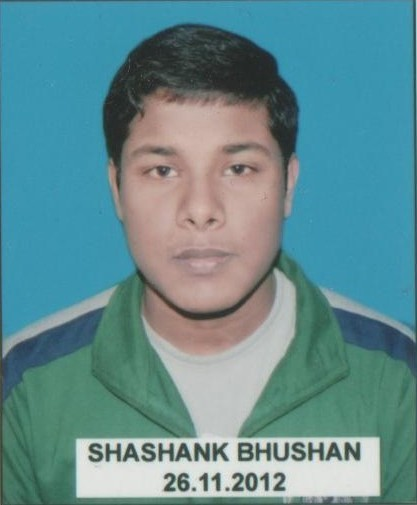
\includegraphics[height=3.5cm , width=2.8cm]{Bhushan.jpg}
% \end{wrapfigure}

{\noindent\uppercase{\textbf{\LARGE{Neha Mishra}}}\\}
\\
\hspace{73pt}Third Year Undergraduate\\
\hspace{73pt}Electronics and Communication Engineering \\
\hspace{73pt} Email ID: \runlocation{\href{mailto:skbhu@iitk.ac.in}{skbhu@iitk.ac.in}} \\
Mobile No: +91-7754915990\\
Address: \textbf{Room No. 276, Hall of Residence 3, IIT Kanpur, Uttar Pradesh}\\
\microspace
\noindent\makebox[\linewidth]{\color{headings}\rule{\paperwidth}{0.6pt}} % Horizontal rule
\vspace{-5pt}

%
%----------------------------------------------------------------------------------------
%	RIGHT COLUMN
%----------------------------------------------------------------------------------------
%
\begin{minipage}[t]{1.00\textwidth} % The right column takes up 66% of the text width of the page
%------------------------------------------------
% Education
%------------------------------------------------

{\uppercase\uline{\textbf{\large{Interests}}\hfill}\\}
\microspace
Startups \& Entrepreneurship, Android Development, Graphics Designing, Data Structures \& Algorithms
\microspace

{\uppercase\uline{\textbf{\large{Education}}\hfill}\\}

\begin{tabular}{|l|l|l|l|}
\cline{1-4}
\textbf{Year}&\textbf{Degree}&\textbf{Institute}&\textbf{CPI/\%}\\
\cline{1-4}
2017(expected)&Bachelor of Technology&Indian Institute of Technology Kanpur&5.7*/10.0\\
2012&All India Senior School Certificate Examination (CBSE)&Shiv Jyoti , Kota&73.4 \%\\
2010&Indian Certificate of Secondary Education (ICSE)&Don Bosco Academy, Patna&82 \%\\
\cline{1-4}
\end{tabular}
\microspace
\hfill{* - \textit{\small{at the end of fourth semester}}}

%------------------------------------------------
% Awards & Acheivements
%------------------------------------------------

{\uppercase\uline{\textbf{\large{Academic  Achievements}}\hfill}}
\begin{tightitemize}
\item Secured \textbf{All India Rank 3429} in JEE Advanced out of more than 500,000 aspirants.\hfill{\textbf{2013}}
\item Secured a \textbf{score of 265/360} in JEE Mains given by around 1,300,000 students.\hfill{\textbf{2013}}
\item Secured a \textbf{score of 382/450} in BITS Entrance Exam.\hfill{\textbf{2013}}
\end{tightitemize}

\sectionspace % Some whitespace after the section

%------------------------------------------------
% Experience
%------------------------------------------------

{\uppercase\uline{\textbf{\large{Work Experience}}\hfill}}
\microspace

\runsubsection{CRANKOUT TECH Pvt Ltd}
\rundescript{| Android App Development Intern}
\hfill {\textbf{(May 2015-Jul 2015)}}\\
\location{Book Any Gym, Studio, Sports venue or personal Health Coach in Mumbai.(\href{http://www.crankoutapp.com/}{CrankOut App})}

\begin{tightitemize}
\item Created a minimalistic flow and paid special attention to user experience , made booking easy enough so that any person can fluently use all the services .
\item Implemented Session Management, Cart Management and Material Design guidelines.
\end{tightitemize}

\sectionspace % Some whitespace after the section

%--------------------------------------------------------------------

{\uppercase\uline{\textbf{\large{Projects}}\hfill}}
\microspace

\runsubsection{Auraplay - An Articulated Mechanical Robotic Arm}
\rundescript{| Electronics Club Project }
\hfill {\textbf{(May 2014-Jun 2014)}}\\

\begin{tightitemize}
\item Making a Fluid Interface controlled by laser pen which is a projected screen.\runlocation{\href{https://www.youtube.com/watch?v=5coxYI7yprY}{(Project Video Link)}}
\item Using OpenCV to track screen through contour detection and mouse handling trough laser . Using this mouse you can move screen any place on a table top.
\item Servo motors and Arduino was used to make the 2DOF movement of the robotic arm using wiring pi libraries.
\end{tightitemize}

\microspace

\runsubsection{TA202}
\rundescript{| Course Project under Prof. V.K. Jain }
\hfill {\textbf{(Jan 2015-Apr 2015)}}\\
\begin{tightitemize}
\item A Fully Functional Automatic wheat plant sowing machine was made by a group of 6 people and was awarded as the \textbf{best project} from the whole batch of 440 students.
\item The mechanism was designed such that the whole machine could be driven from a single point's motion .\runlocation{\href{https://www.youtube.com/watch?v=kp_Sz-XeJyE}{(Project Video Link)}}
\item Using Matlab stimulation to calculated the trajectory of the end points in a 4 bar mechanism to make picking effective.
\end{tightitemize}

\microspace

\runsubsection{TA201}
\rundescript{| Course Project under Prof. Shashank Shekhar }
\hfill {\textbf{(Aug 2014-Nov 2014)}}\\
\begin{tightitemize}
\item Made a model to demonstrate the Perpetual Motion , and hence demonstrate the first and second law of thermodynamics.
\item Using Manufacturing processes with careful precision like welding , molding etc to make a wheels with attached bars to it.
\end{tightitemize}

\microspace

\runsubsection{LINE FOLLOWING ROBOT}
\rundescript{| A seven sensor PID line Following bot | Takneek ( IITK Intra college Techfest)}
\hfill {\textbf{(Aug 2014)}}\\
\begin{tightitemize}
\item Made a black line following robot using a seven sensor array , and working with arduino to programme it to implement Proportional – Integral – Derivative(PID) for smooth following.
\end{tightitemize}

\sectionspace
%------------------------------------------------
% Technical Skills
%------------------------------------------------

{\uppercase\uline{\textbf{\large{Technical Skills}}\hfill}}

\begin{tightitemize}
\item \textbf{Programming Languages :  }C, C++, JavaScript
\item \textbf{Web Development \hspace{28pt}: } HTML, CSS, Django, Node.js, Bootstrap.css, MongoDB
\item \textbf{Utilities \& Softwares \hspace{19pt}: } Git, Make, Bash, Postman, Microsoft Excel, Microsoft PowerPoint
\item \textbf{Operating Systems \hspace{27pt}: } Fedora, Ubuntu, Mac OS, Windows
\item \textbf{Design Software \hspace{28pt}:} Sketch(Mac) , Auto-cad , Solidworks Autodesk Inventor , Adobe Illustrator ,Adobe Photoshop
\end{tightitemize}
\sectionspace
%------------------------------------------------
% Coursework
%------------------------------------------------

{\uppercase\uline{\textbf{\large{Relevant Coursework}}\hfill}}

\runlocation{Mechanical Engg.} : Engineering Design and Graphics,Nature and Properties of Material, Fluid Mechanics, Graphical Engineering,\\
	    	\hspace{83pt}  Manufacturing Processes, Dynamics\textbf{*} , Mechanics Of Solids\textbf{*}, Energy Systems\textbf{*}\\
		\hspace{83pt} Manufacturing Science and Technology\textbf{*} , \\
\runlocation{Others}\hspace{46pt} : Fundamentals of Computing, Complex Variables , Introduction to Electrical Engineering,\\ 
		\hspace{83pt} Partial Differential Equations, Introduction to Electronics, Flight Mechanics\textbf{*} \hfill {\small \textbf{(* - ongoing)}}\\

\sectionspace % Some whitespace after the section


\end{minipage} % The end of the right column

%----------------------------------------------------------------------------------------
%	LEFT COLUMN
%----------------------------------------------------------------------------------------

\begin{minipage}[t]{1.00\textwidth} % The left column takes up 33% of the text width of the page

%------------------------------------------------
% Leadership Skills
%------------------------------------------------

{\uppercase\uline{\textbf{\large{Leadership Skills}}\hfill}}

\microspace
\rundescript{{CULTURAL SECRETARY} | Hall Executive Committee, Hall 3}
\hfill {\textbf{(Jul 2014-Apr 2015)}}\\
\begin{tightitemize}
\item Was part of a team of 11 people who managed all the Hall level Activities and supervised inter as well as intra-hall events.
\item Won the Galaxy trophy for the 7th time in a row which is IITK's inter-hall cultural Festival.
\item Invented a programme through which every new resident of the hall could get full exposure to cultural activities.
\end{tightitemize}

\minispace

\rundescript{COORDINATOR – INFORMALS , TECHKRITI'15 ( Technical and Entrepreneurship Festival of IIT Kanpur )}
\hfill {\textbf{(Mar 2015)}}\\
\begin{tightitemize}
\item Organised and Invented Ideas for Fun Games which was open to all present in the Techkriti.
\item As well as secured the online points portal from being hacked.
\end{tightitemize}

\minispace

\rundescript{COORDINATOR – DESIGN EVENTS , TECHKRITI'15}
\hfill {\textbf{(Mar 2015)}}\\
\begin{tightitemize}
\item Conducted the competitions of Techkriti grand prix and Concantenate in our technical fest which included bringing partications from over India
\item Emphasised on post festival logistics management reduce the lead time from 5 months to 2 months.
\end{tightitemize}

\minispace

\rundescript{SECRETARY ELEVATOR PITCH – BUISENESS EVENTS , TECHKRITI'14}
\hfill {\textbf{(Mar 2014)}}\\
\begin{tightitemize}
\item Managed the Operations of event and Conducted it and won a price for participation as an audience.
\end{tightitemize}

\minispace

{\uppercase\uline{\textbf{\large{Hobbies}}\hfill}\\}

\microspace
Staying Updated with Technical Entrepreneur Events, Traveling, Management of Events, Cooking 
\microspace

%----------------------------------------------------------------------------------------

\end{minipage} % The end of the left column
\hfill

%----------------------------------------------------------------------------------------
%	SECOND PAGE (EXAMPLE)
%----------------------------------------------------------------------------------------

%\newpage % Start a new page

%\begin{minipage}[t]{0.33\textwidth} % The left column takes up 33% of the text width of the page

%\section{Example Section}

%\end{minipage} % The end of the left column
%\hfill
%\begin{minipage}[t]{0.66\textwidth} % The right column takes up 66% of the text width of the page

%\section{Example Section 2}

%\end{minipage} % The end of the right column

%----------------------------------------------------------------------------------------

\end{document}
